\documentclass[conference]{IEEEtran}
\IEEEoverridecommandlockouts
\usepackage{matlab-prettifier}
\usepackage{cite}
\usepackage{amsmath,amssymb,amsfonts}
\usepackage{nccmath}
\usepackage{algorithmic}
\usepackage{graphicx}
\usepackage{textcomp}
\usepackage{xcolor}
\usepackage{float}
\usepackage{tabularx}
\def\BibTeX{{\rm B\kern-.05em{\sc i\kern-.025em b}\kern-.08em
    T\kern-.1667em\lower.7ex\hbox{E}\kern-.125emX}}

%\renewenvironment{align*}{\par$\!\aligned}{\endaligned$\par}

%\setlength{\mathindent}{1cm}

\begin{document}

\title{Project 1 : Matched Filtering of an LFM Waveform}

\author{\IEEEauthorblockN{Owen Sowatzke}
\IEEEauthorblockA{\textit{Electrical Engineering Department} \\
\textit{University of Arizona}\\
Tucson, USA \\
osowatzke@arizona.edu}}
\maketitle

\begin{abstract}
The range resolution of a rectangular pulse is inversely proportional to the length of the rectangular pulse. Therefore, to achieve fine range resolution, a short rectangular pulse is required. However, decreasing the pulse length also leads to a reduction in SNR. Pulse compression waveform seek to decouple pulse length from range resolution and in turn make it possible to simultaneously achieve fine range resolution and a high SNR. One common pulse compression waveform is a linear frequency modulated (LFM) waveform. This document simulates the matched filer response of an LFM waveform and examines the resulting SNR and range resolution.
\end{abstract}

\begin{IEEEkeywords}
Pulse Compression, Linear Frequency Modulated (LFM) Waveform, Matched Filter
\end{IEEEkeywords}
\section{Introduction}
A linear frequency modulated (LFM) waveform is a pulse compression waveform defined by the following equation:
\begin{equation}
x(t)=e^{j\pi\beta t^2/\tau}
\label{lfm_waveform}
\end{equation}
where:
\begin{fleqn}[\parindent]
\begin{align*}
\beta &= \text{Waveform Bandwidth (Hz)}\\
\tau &= \text{Waveform Duration (s)}
\end{align*}
\end{fleqn}
A sample pulsed radar system will be created in MATLAB to simulate the matched filter response of this waveform. Using the radar system model, the SNR of the matched filter output will be measured and compared to the SNR of the input signal. Additionally, multiple target returns will be generated and used to measure the system's range resolution.
\section{Sample Radar System Parameters}
To generate the required matched filter response, a pulsed radar system was simulated in MATLAB using the following set of parameters: 
%The pulse radar system simulated in MATLAB was designed with the following set of parameters: 
\begin{table}[H]
\caption{Radar System Parameters}
\label{Parameter Table}
\begin{tabularx}{0.5\textwidth}{| X | X |}
\hline
Carrier Frequency & 10 GHz \\
\hline
Sample Rate & 100 MHz \\
\hline
Transmit Power & 20 dB \\
\hline
Antenna Gain & 44.15 dB \\
\hline
Noise Figure & 10 dB \\
\hline 
System Losses & 5 dB \\
\hline
PRF & 50 kHz \\
\hline
Duty Cycle & 20\% \\
\hline
Chirp Bandwidth & 100 MHz \\
\hline
\end{tabularx}
\end{table}
\noindent
Additional parameters can be computed using the parameters given in Table \ref{Parameter Table}. For example, the radar system's PRI can be computed as follows:
\begin{equation}
PRI = \frac{1}{PRF} = 20 {\mu}s
\label{PRI Equation}
\end{equation}
Another parameter of interest, the length of the LFM pulse ($\tau$), can be computed using the duty cycle ($D$) as follows:
\begin{equation}
\tau = PRI \cdot D = 4 {\mu}s
\label{tau equation}
\end{equation}
\section{Modeling the Matched Filter Output}
\label{modeling_section}
To model the matched filter response of the system, the received signal must first be generated for each of the target returns. The process of generating the received signal is illustrated in Fig. \ref{gen_rx_sig}.
\begin{figure}[H]
\centerline{\fbox{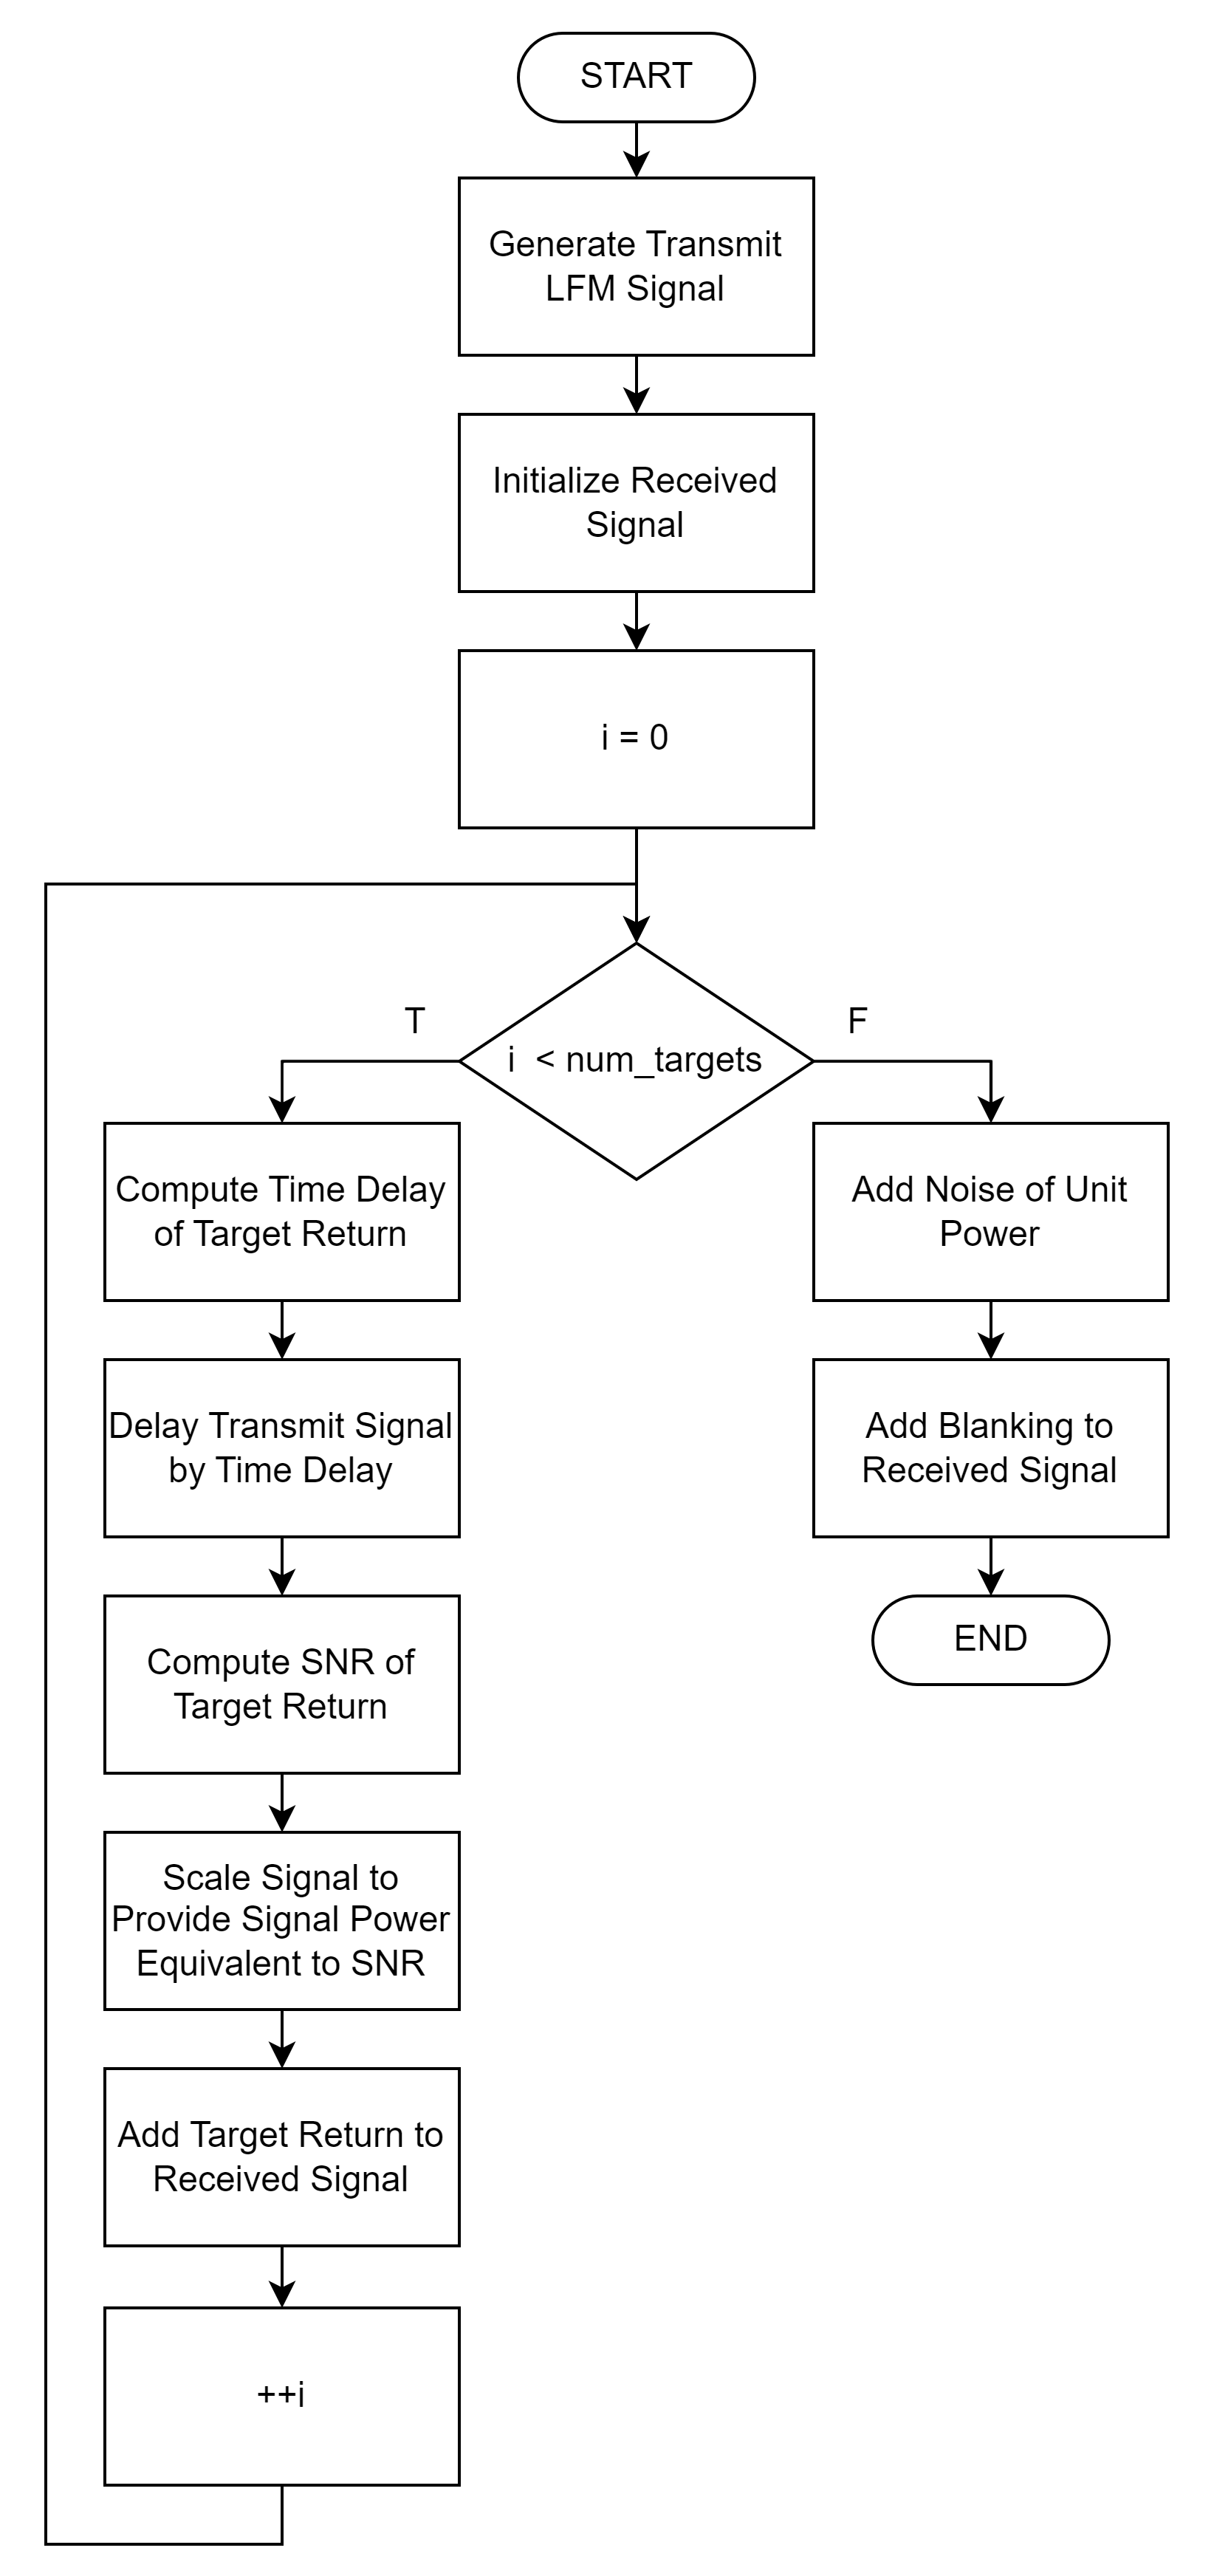
\includegraphics[width=0.3\textwidth]{gen_rx_sig.png}}}
\caption{Generating the Received Signal.}
\label{gen_rx_sig}
\end{figure}
Each of the target returns is a delayed and scaled version of the transmitted signal. As such, the transmitted LFM waveform must be generated as part of the workflow. This is done using equation \eqref{lfm_waveform}. Note that the transmitted signal must be padded with zeros to account for the listening period after transmission.
\par
For a target at a range of $R$ meters, the transmitted signal is delayed by
\begin{equation}
t_d = \frac{R}{2c} \enspace s
\end{equation}
The SNR of the target return is given by the following equation:
\begin{equation}
SNR = \frac{P_t G^2 \lambda^2 \sigma}{(4\pi)^3 R^4 k T_0 B_n F_n L_s L_\alpha(R)}
\label{snr_formula}
\end{equation}
To create a target return with the desired SNR, either the signal power or noise power can be scaled. For this simulation, the signal power is scaled while the noise power is held constant. The transmitted signal given in equation \eqref{lfm_waveform} has unit amplitude, and the noise is sampled from the standard complex normal distribution. Therefore, to achieve the desired SNR, the target return must be scaled by the following factor:
\begin{equation}
k = 10^{SNR(dB)/20}
\end{equation}
\par
The received signal is the sum of each target return and noise. During waveform transmission, the receiver is assumed to be "blanked" (i.e. it cannot listen while transmitting). To model the effects of "blanking", the beginning of the received pulse is replaced with zeros.
\par
To increase the SNR of the received signal, the signal is passed through a matched filter. The radar system's matched filtering process is shown in Fig. \ref{gen_mf_output}. 
\begin{figure}[H]
\centerline{\fbox{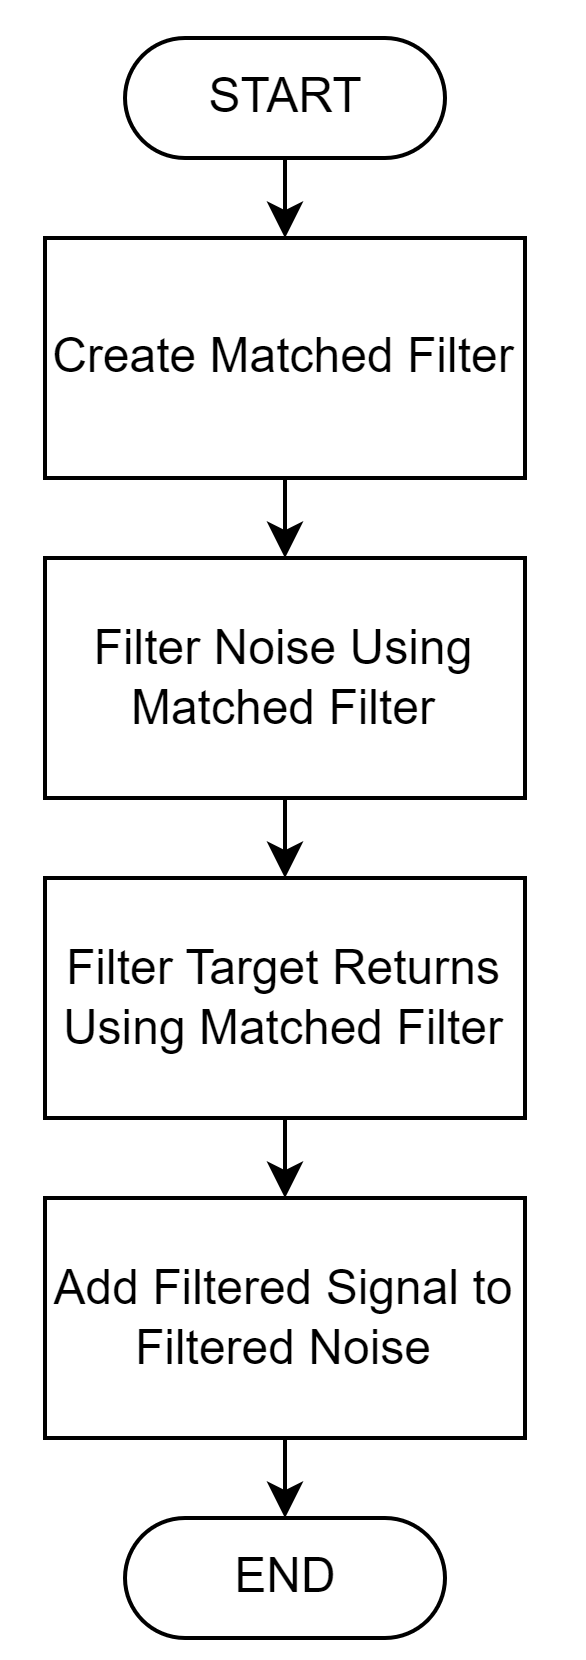
\includegraphics[width=0.15\textwidth]{gen_mf_output.png}}}
\caption{Matched Filtering of the Input Signal.}
\label{gen_mf_output}
\end{figure}
\par
The system's matched filter is generated using to the following equation:
\begin{equation}
h = x^*(T_M-t)
\end{equation}
To ensure the matched filter is causal, $T_M$ is chosen to be the length of the transmitted LFM waveform.
\par
In the radar system model, both the noise and target returns are filtered independently. Note that this provides the same result as directly filtering the received signal.
\begin{equation}
y(t) = h(t)*(x(t)+n(t)) = h(t)*x(t) + h(t)*n(t)
\end{equation}
However, it also provides the ability to easily extract signal and noise power measurements from the matched filter output.
\section{Matched Filter Output SNR}
\label{mf_snr_section}
The SNR at the output of the matched filter output should be greater than the SNR of the received signal by a factor of $L$, where $L$ is the matched filter length in samples. For the given radar system, the matched filter length is
\begin{equation}
L = \frac{\tau}{T_s} = \tau f_s = 400 \text{ samples}
\end{equation}
Therefore, the SNR of the matched filter output should be $10log_{10}(400)=26.02 \text{ dB}$ greater than that of the received signal. This result will be confirmed via simulation.
\par
To simulate the matched filter response of the system, a target is placed in the first ambiguity at a range corresponding to a time delay of 25\% of the PRI. The resulting range is
\begin{equation}
R = \frac{ct_d}{2} = 750 \text{ m}
\label{tgt1 range}
\end{equation}
The RCS of the target can be calculated to provide an arbitrary SNR at the ADC. Starting with equation \eqref{snr_formula}, the RCS can be expressed in the following form:
\begin{equation}
\sigma = \frac{(4\pi)^3 R^4 k T_0 B_n F_n L_s L_\alpha(R)\cdot SNR}{P_t G^2 \lambda^2}
\label{rcs_formula}
\end{equation}
For this system, the SNR at the ADC is chosen to be 20 dB. This SNR corresponds to a RCS of $0.01307m^2$.
\par
The received signal for this target configuration can be generated according to Section \ref{modeling_section}. The resulting ADC signal is shown in Fig. \ref{adc_sig}.
\begin{figure}[H]
\centerline{\fbox{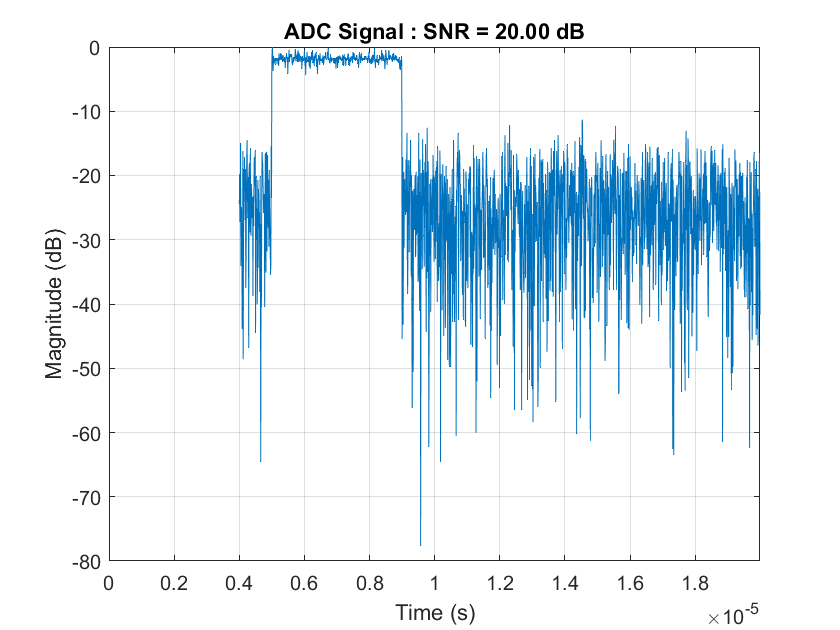
\includegraphics[width=0.4\textwidth]{adc_sig.png}}}
\caption{Received ADC Signal.}
\label{adc_sig}
\end{figure}
\noindent
This ADC signal can be then passed through the system's matched filter to produce the plot shown in Fig. \ref{mf_output}.
\begin{figure}[H]
\centerline{\fbox{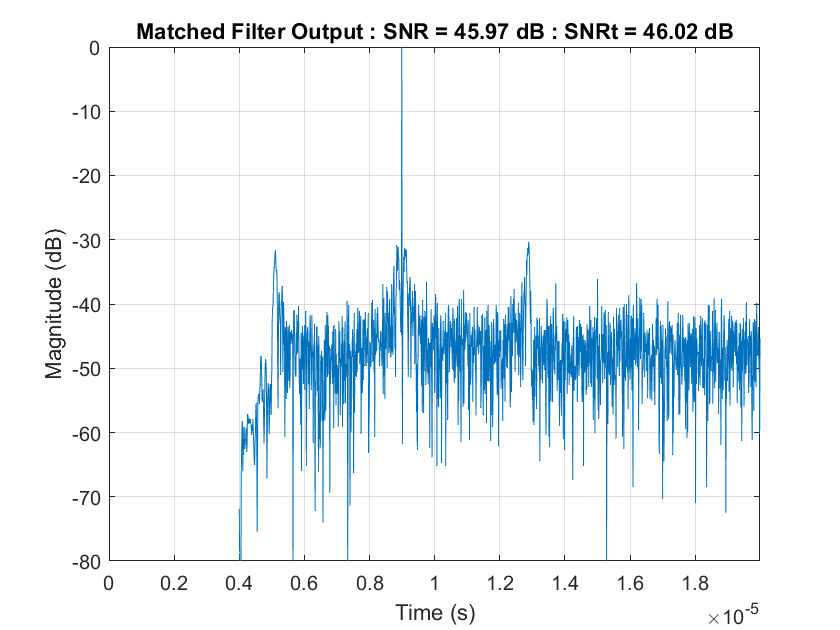
\includegraphics[width=0.4\textwidth]{mf_output.png}}}
\caption{Matched Filter Output.}
\label{mf_output}
\end{figure}
\noindent
The SNR of the matched filter output is given by the following equation:
\begin{equation}
SNR = 10log_{10}\frac{P_s}{P_n}
\end{equation}
where:
\begin{fleqn}[\parindent]
\begin{align*}
P_s &= \text{Signal Power}\\
P_n &= \text{Noise Power}
\end{align*}
\end{fleqn}
The resulting signal power is defined using the peak of the filtered target return as follows:
\begin{equation}
P_s = \text{max(}|x[k]|\text{)}^2
\end{equation}
The resulting noise power is defined using the filtered noise samples ($n[k]$). Note that the first $2L-1$ noise samples are ignored due to "blanking" and the "charge-up" of the matched filter. Let $m \in [0, N)$ be the "charged-up" samples of the matched filter. Then, the noise power is given by
\begin{equation}
P_n = \frac{1}{N}\sum_{m=0}^{N-1}|n[m]|^2
\end{equation}
\par
For the given simulation, the observed SNR at the matched filter output is $45.97 \text{ dB}$. Note that this is approximately equivalent to the expected SNR of $46.02 \text{ dB}$.
\section{Matched Filter Range Resolution} 
The range resolution of the matched filter output is theoretically given by
\begin{equation}
\Delta R = \frac{c}{2\beta}
\end{equation}
This result will be confirmed via simulation. First, a target will be placed as described in Section \ref{mf_snr_section}. Then, a second target will be placed at a larger range and moved toward the first target until the two targets are indistinguishable from each other. 
\par
To start, the second target was placed two code lengths ($2L$ samples) away from the first target. This guarantees that the matched filter responses from each target return are non-overlapping. The resulting range of the second target is given by
\begin{equation}
R = 750 + \frac{c(2\tau)}{2} = 750 + c\tau = 1950 \text{ m}
\end{equation}
The SNR of the second target return is configured to be 20 dB. Using equation \eqref{rcs_formula}, the resulting RCS is given by $0.59758m^2$. The matched filter response for the combined target return is shown in Fig. \ref{mf_output_clearly_resolvable}.
\begin{figure}[H]
\centerline{\fbox{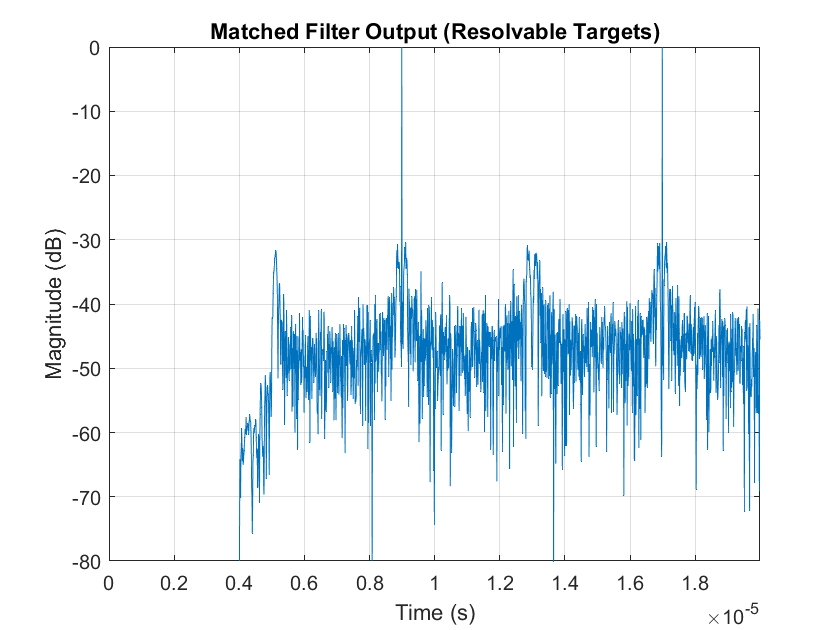
\includegraphics[width=0.4\textwidth]{clearly_resolvable.png}}}
\caption{Resolvable Target Returns ($1200$m Spacing).}
\label{mf_output_clearly_resolvable}
\end{figure}
\par
The second target is clearly distinguishable from the first. As such, the second target can be moved significantly closer to the first target. If it is placed 2 ADC samples away from the first target, the resulting range is given by
\begin{equation}
R = 750 + \frac{c(2T_s)}{2} = 750 + cT_s = 753 \text{ m}
\end{equation}
The SNR of this target return can be configured as 20 dB. This results in an RCS of $0.01328m^2$. The matched filter response resulting from the updated target returns is shown in Fig. \ref{resolvable_full}.
\begin{figure}[H]
\centerline{\fbox{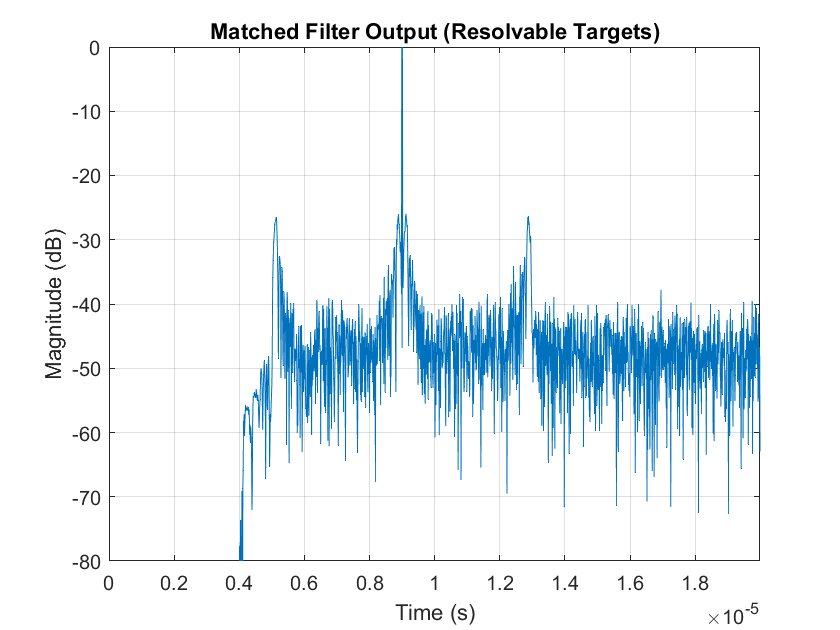
\includegraphics[width=0.4\textwidth]{resolvable_full.png}}}
\caption{Resolvable Target Returns ($3$m Spacing).}
\label{resolvable_full}
\end{figure}
\noindent
After zooming in on the peak of the matched filter response, the targets can easily be resolved. This is shown in Fig. \ref{resolvable_peak}.
\begin{figure}[H]
\centerline{\fbox{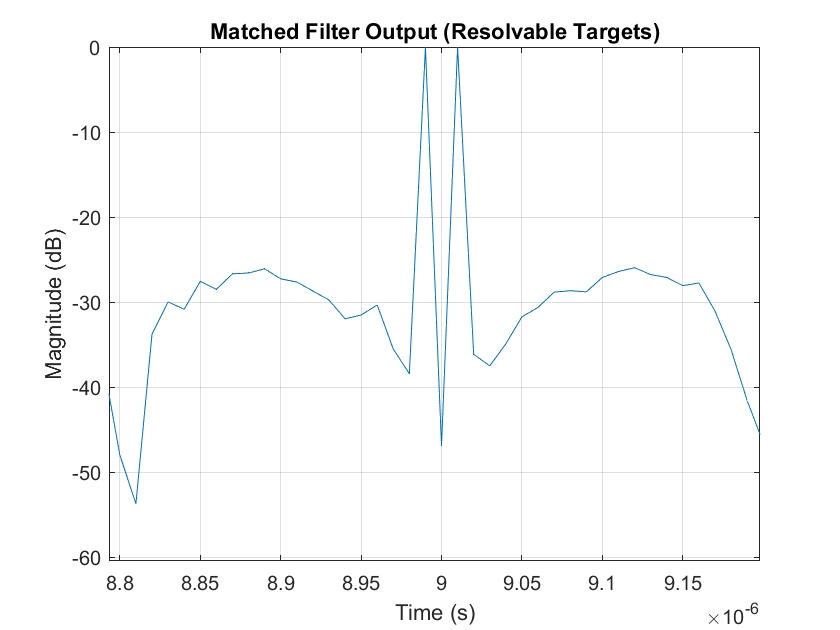
\includegraphics[width=0.4\textwidth]{resolvable_peak.png}}}
\caption{Resolvable Target Returns ($3$m Spacing).}
\label{resolvable_peak}
\end{figure}
\par
If the second target is moved one sample closer to the first target, the range of the second target is given by 
\begin{equation}
R = 750 + \frac{cT_s}{2} = 751.5 \text{ m}
\end{equation}
If the SNR of the target is configured as 20 dB, the resulting RCS is given by $0.01307m^2$. The peak of the updated matched filter is shown in Fig. \ref{unresolvable_peak}.
\begin{figure}[H]
\centerline{\fbox{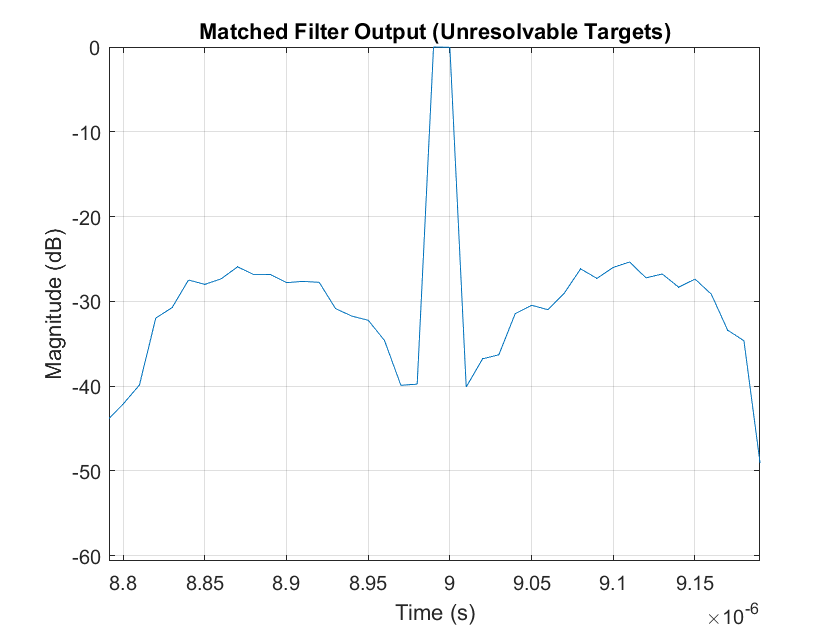
\includegraphics[width=0.4\textwidth]{unresolvable_peak.png}}}
\caption{Unresolvable Target Returns ($1.5$m Spacing).}
\label{unresolvable_peak}
\end{figure}
\par
Note that the target returns have blurred into a single target return. Therefore, the resulting range resolution is $1.5 \text{ m}$. 
%The resulting matched filter output can then be used to draw conclusions about SNR and range resolution.
% 
%The matched filter response of the radar system can be generated by modeling the signal from the DAC to the matched filter. modeling the radar signal from the tranmission matched filter. 

%\section{Introduction}
%Both Monte Carlo (MC) Simulations and Importance Sampling (IS) are techniques for estimating probabilities. In this document, both techniques will be used to estimate the probability that a random variable $X$ with distribution $X\sim N(1,1)$ exceeds 3.957 (i.e. $P\{X > 3.957\}$).
%\section{Monte Carlo Simulation}
%The probability of interest can be written as follows:
%\begin{equation}
%P\{X > 3.957\} = \int_{-\infty}^{\infty}I(x)f_X(x)dx
%\label{Pint}
%\end{equation}
%where
%\begin{equation}
%I(x) = \begin{cases}
%1 & x > 3.957 \\
%0 & x \leq 3.957
%\end{cases}
%\label{Ix_def}
%\end{equation}
%Note that this probability can also be written as an expected value:
%\begin{equation}
%P\{X > 3.957\} = E[I(X)]
%\end{equation}
%Monte Carlo Simulation attempts to estimate this probability using a sample mean
%\begin{equation}
%P\{X > 3.957\} \approx \frac{1}{N}\sum_{i=1}^{N}I(x_i)
%\end{equation}
%where
%\begin{equation}
%x_1, x_2, ..., x_N \sim f_X(x)
%\end{equation}
%\par
%Given different values of $N \in [1, 10^5]$, Monte Carlo Simulations can be used to estimate $P\{X > 3.957\}$. This estimate can than be compared to the true probability.
%\begin{equation}
%P\{X > 3.957\} = 0.001553
%\end{equation}
%The Monte Carlo probability estimate was generated for values $N$ from $100$ to $10^5$ in increments of $100$. The MATLAB code to generate this estimate is included in Appendix \ref{matlab_code}. The Monte Carlo probability estimate is plotted vs $N$ in Fig. \ref{Monte Carlo Estimate}
%\begin{figure}[H]
%\centerline{\includegraphics[width=0.5\textwidth]{Monte_Carlo_Estimate.png}}
%\caption{Monte Carlo Probability Estimate}
%\label{Monte Carlo Estimate}
%\end{figure}
%\noindent
%The absolute value of the error between the Monte Carlo estimate and the true probability ($|P_{est}\{X > 3.957\} - P_{truth}\{X > 3.957\}|$) is also plotted vs $N$.
%\begin{figure}[H]
%\centerline{\includegraphics[width=0.5\textwidth]{Monte_Carlo_Error.png}}
%\caption{Monte Carlo Probability Error}
%\label{Monte Carlo Perr}
%\end{figure}
%As $N\rightarrow\infty$, the Monte Carlo Estimate should approach the true probability. This is confirmed by the reduction in variance as $N$ increases in Fig. \ref{Monte Carlo Perr}.
%\section{Importance Sampling}
%Examining the shaded area in Fig. 
%\ref{Monte Carlo Limits}, very few of the samples used in the Monte Carlo estimate actually lie within the shaded region. This  leads to large variances in the Monte Carlo probability estimates.
%\begin{figure}[H]
%\centerline{\includegraphics[width=0.5\textwidth]{Monte_Carlo_Limitations.png}}
%\caption{Computing Probability from $f_X(x)$}
%\label{Monte Carlo Limits}
%\end{figure}
%Importance Sampling attempts to overcome these limitations. It re-expresses equation \eqref{Pint} in the following form:
%\begin{equation}
%P\{X > 3.957\} = \int_{-\infty}^{\infty}I(x)f_X(x)\frac{g_X(x)}{g_X(x)}dx
%\label{is_int}
%\end{equation}
%where $I(x)$ is given by equation \eqref{Ix_def}.
%Equation \eqref{is_int} can be written as follows:
%\begin{equation}
%P\{X > 3.957\} = \int_{-\infty}^{\infty}I(x)\frac{f_X(x)}{g_X(x)}g_X(x)dx
%\end{equation}
%This equation can also be written as an expected value.
%\begin{equation}
%P\{X > 3.957\} = E\left[I(x)\frac{f_X(x)}{g_X(x)}\right]
%\end{equation}
%Once again, the expected value can be estimated using sample mean.
%\begin{equation}
%P\{X > 3.957\} \approx \frac{1}{N}\sum_{i=1}^{N}I(x_i)\frac{f_X(x_i)}{g_X(x_i)}
%\end{equation}
%Note the samples $x_1,x_2,...,x_N$ are sampled from $g_X(x)$ instead of $f_X(x)$. This enables us to select a density $g_X(x)$ with more "important" samples. 
%\par
%Consider a density $g_X(x)$ that is a shifted version of $f_X(x)$. Specifically, consider the following density function
%\begin{equation}
%g_X(x) = \frac{1}{\sqrt{2\pi}}e^{-(x-3.957)^2/2}
%\end{equation}
%The important samples of this density function are highlighted in Fig. \ref{Important Samples}. 
%\begin{figure}[H]
%\centerline{\includegraphics[width=0.5\textwidth]{Important_Samples.png}}
%\caption{Important Samples from $g_X(x)$}
%\label{Important Samples}
%\end{figure}
%\noindent
%Note that the number of important samples is significantly larger than that of Fig. \ref{Monte Carlo Limits}. This should reduce the variance of the probability estimate. 
%\par
%The Importance Sampling probability estimate was generated for values $N$ from $100$ to $10^5$ in increments of $100$. The MATLAB code to generate this estimate is included in Appendix \ref{matlab_code}. The Important Sampling probability estimate is plotted vs $N$ in Fig. \ref{Importance Sampling Estimate}.
%\begin{figure}[H]
%\centerline{\includegraphics[width=0.5\textwidth]{Importance_Sampling_Estimate.png}}
%\caption{Importance Sampling Probability Estimate}
%\label{Importance Sampling Estimate}
%\end{figure}
%\noindent
%The absolute value of the error between the Importance Sampling estimate and the true probability ($|P_{est}\{X > 3.957\} - P_{truth}\{X > 3.957\}|$) is also plotted vs $N$.
%\begin{figure}[H]
%\centerline{\includegraphics[width=0.5\textwidth]{Importance_Sampling_Error.png}}
%\caption{Importance Sampling Probability Error}
%\label{Importance Sampling Perr}
%\end{figure}
%The variance of the Monte Carlo and Importance Sampling probability estimates can be compared by overlaying the probability error plots. This plot is shown in Fig. \ref{Error Overlay}
%\begin{figure}[H]
%\centerline{\includegraphics[width=0.5\textwidth]{Error_Overlay.png}}
%\caption{Probability of Error Comparison}
%\label{Error Overlay}
%\end{figure}
%\noindent
%Note that the Importance Sampling probability estimate is much closer to the expected probability than the Monte Carlo Estimate. As such, the Importance Sampling estimate has a much lower variance for the same values of $N$.
%\section{Conclusion}
%Monte Carlo Simulation and Importance Sampling are ways to estimate probabilities. Both of these approaches were used to estimate $P\{X > 3.957\}$ for $X \sim N(1,1)$. As demonstrated, importance sampling produced a probability estimate with a smaller variance than that of Monte Carlo simulation. This result can be applied to other probabilities estimates as well. If a distribution is hard to sample, importance sampling can be used to reduce the number of samples required to produce an estimate. This can make a significant difference, especially when it is computationally intensive to determine if the random variable exceeds the threshold.
%\onecolumn
%\pagebreak
%\appendices
%\section{MATLAB Source Code}
%\label{matlab_code}
%\lstset{style=Matlab-editor}
%\lstinputlisting{Project3_Sowatzke.m}
%\raggedbottom
\end{document}
